\documentclass[10pt]{article}

\usepackage[utf8x]{inputenc}
\usepackage[T1]{fontenc}
\usepackage[finnish]{babel}
\usepackage{amsmath}
\usepackage{amssymb}
\usepackage{amsfonts}
\usepackage{amsthm}
\usepackage{graphicx}
\usepackage[ruled]{algorithm2e}
\usepackage{empheq}
\usepackage{float}
\usepackage{graphicx}

\title{Tietokantasovellus -- Dokumentaatio}
\date{2014, periodi 4}
\author{Rodion ``rodde'' Efremov}
\renewcommand*\rmdefault{iwona}

\begin{document}
\pagenumbering{Roman}
\maketitle
\newpage
\tableofcontents
\newpage
\pagenumbering{arabic}

\section{Johdanto} Tämä dokumentti on tarkoitettu kuvaamaan Tietokantasovellus-kurssin (582203) aikana toteutettu verkkosovellus. Ajallisesti ottaen kurssisuoritukseni on ajoitettu kevään 2014 neljännelle periodille.

Toteutuskieleksi olen valinnut Javan (servletit Tomcat:n ajettavaksi), ja tietokannaksi olen valinnut niin ikään suositeltu PostgreSQL.

\section{Yleiskuva järjestelmästä}
Aiheenani on keskustelufoorumin toteuttaminen. Järjestelmässä on kolme käyttäjäkategoriaa: 
\begin{itemize}
  \item ylläpitäjä (admin),
  \item moderaattori (moderator),
  \item käyttäjä (user).
\end{itemize}
Käyttäjä voi luoda tunnuksensa rekisteröitymällä sovellukseen. Ensimmäinen ylläpitäjä on luotu SQL-komennosta. Myöhemmin kun järjestelmässä alkaa olla käyttäjiä, ylläpitäjä voi ylentää tavallisen käyttäjän moderaattoriksi tai suoraan ylläpitäjäksi. Lisäksi, ylläpitäjä voi poistaa oman tai mielivaltaisen moderaattorin tai käyttäjän. Mitä tulee tilanteeseen, jossa ylläpitäjä poistaa itseään, onnistuu se vain jos poiston jälkeen järjestelmään jää vähintään yksi muu ylläpitäjä. (Järjestelmässä pitää olla vähintään yksi ylläpitäjä.) Moderaattori voi poistaa käyttäjien viestit, mikäli siihen on tarvetta. Lisäksi, moderaattori voi asettaa käyttäjät maksimissaan 7 vuorokauden käyttökieltoon. Mitä tulee keskustelusäikeisiin, uusien luonti vaatii vähintään moderaattorioikeudet; säikeiden poistaaminen on ainoastaan ylläpitäjien etuoikeus. Ylläpitäjät pystyvät tekemään samat toiminnot kuin moderaattorit.

Mitä tulee itse foorumin rakenteeseen, alkusivulla voi selata ``teemoja''. Jokainen teema pitää sisällään vähintään yhden ``säikeen'', joista jälkimmäinen pitää sisällään siihen liittyvän keskusteluhistorian. Keskustelun lisäksi jokainen käyttäjä/moderaattori/ylläpitäjä voi lähettää yksityiset viestit mielivaltaiselle käyttäjälle ilman statusrajoja.

\section{Käyttötapaukset}
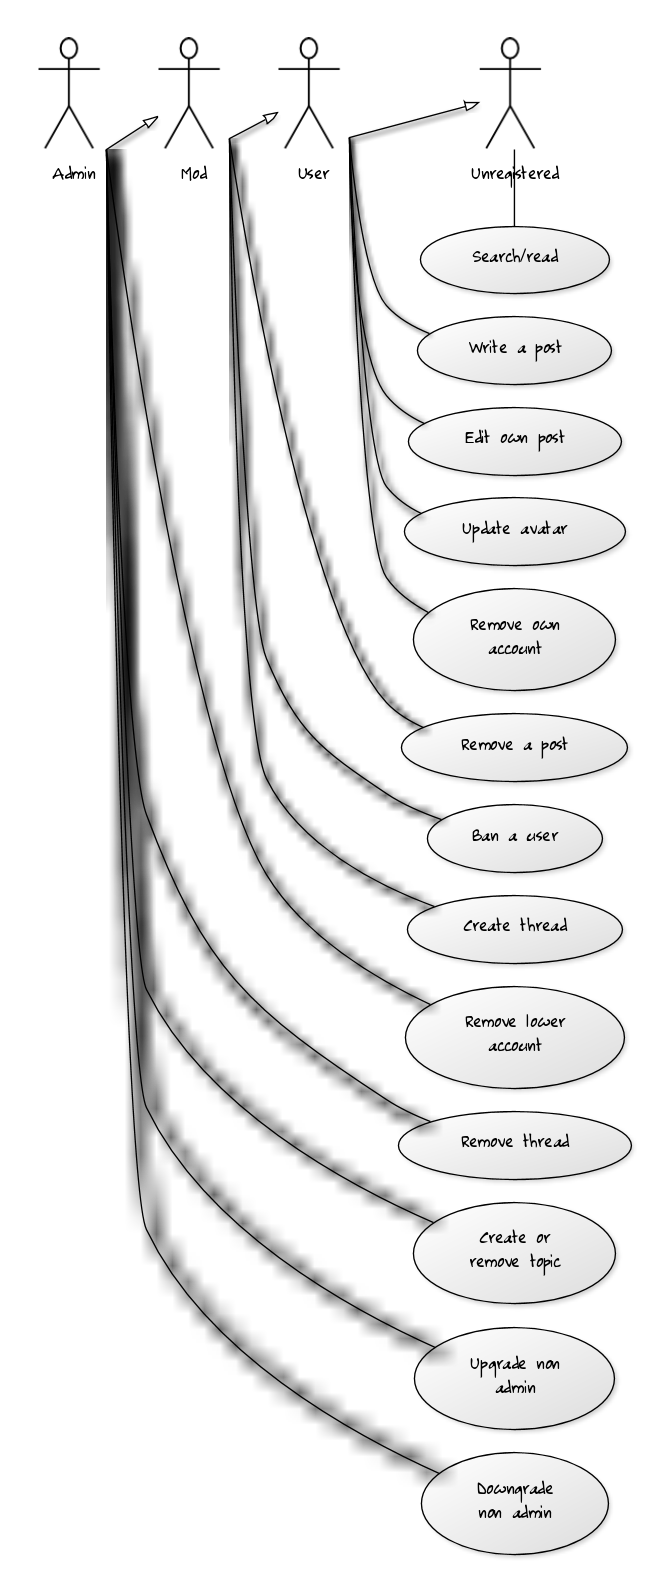
\includegraphics[width=\textwidth]{multilog_use_case_diagram}

\end{document}